\pagebreak
\pagenumbering{Roman}
\section{Anhang}
\subsection{Ergänzende Abbildungen zu Booklet Teil 1}
\label{app:abb_booklet_1}
Folgende Abbildungen stellen die Entscheidungsbäume der Cost-Complexity Aufgabe dar. Der Unterschied in den Bäumen mit geringerem und höherem $\alpha$ wird für die beiden Baum-Variationen gut ersichtlich. Abbildungen \ref{fig:ccp_fulltree_alpha_0005} und \ref{fig:ccp_fulltree_alpha_002} zeigen je einen vollständig ausgebildeten Baum, der durch Cost-Complexity \gqq{beschnitten} wurden.\\
\begin{figure}[H]
    \centering
     \begin{minipage}{0.45\textwidth}
        \centering
        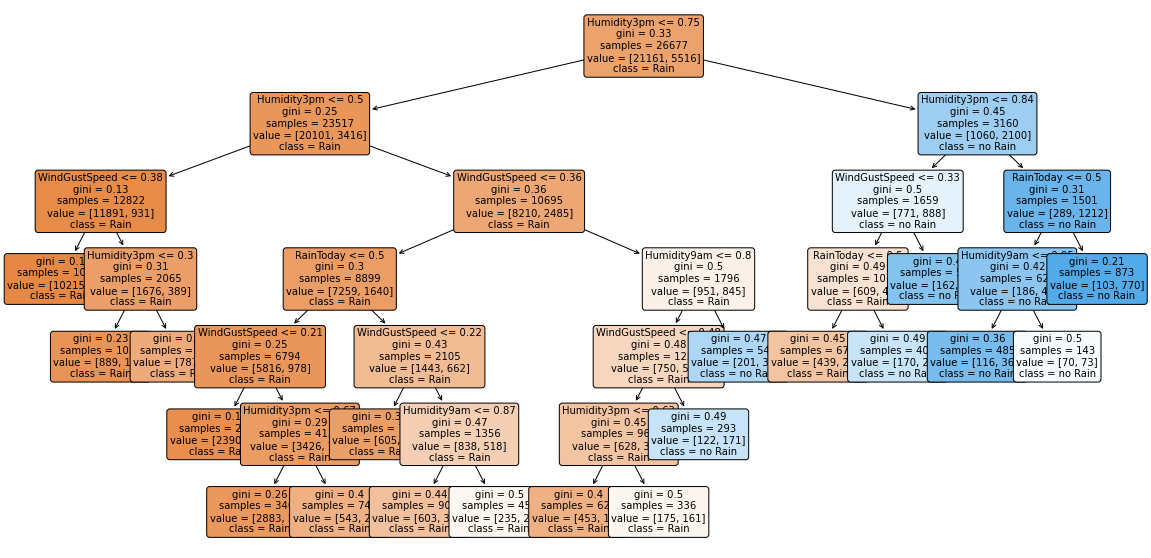
\includegraphics[width=0.9\textwidth]{Bilder/ccp_fulltree_alpha_0005.png}
        \caption{Entscheidungsbaum mit Parametern \emph{max\_depth=None} und \emph{ccp\_alpha=0.0005}}
        \label{fig:ccp_fulltree_alpha_0005}
    \end{minipage}\hfill
    \begin{minipage}{0.45\textwidth}
        \centering
        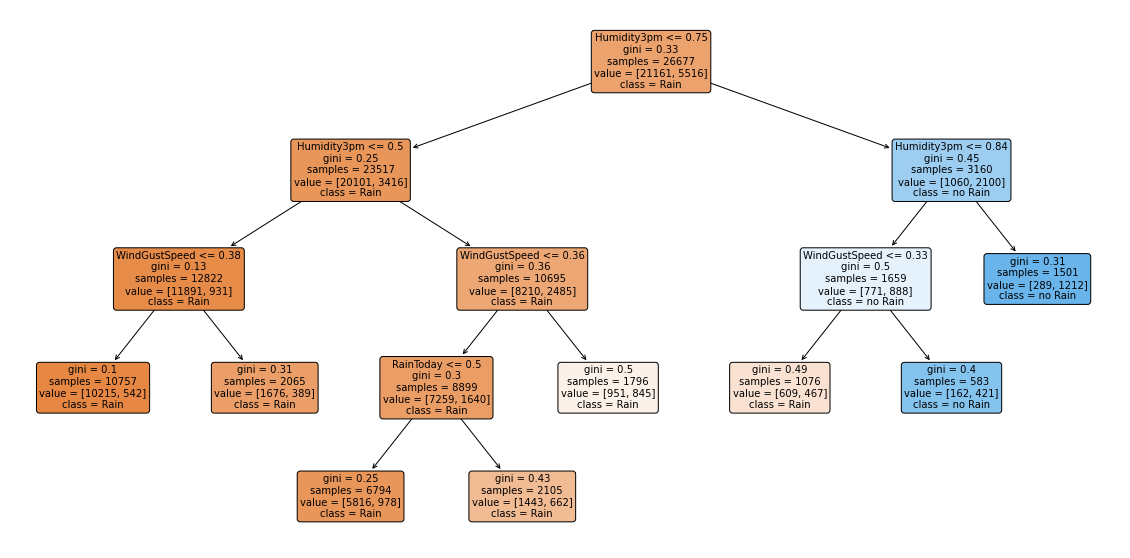
\includegraphics[width=0.9\textwidth]{Bilder/ccp_fulltree_alpha_002.png}
        \caption{Entscheidungsbaum mit Parametern \emph{max\_depth=None} und \emph{ccp\_alpha=0.002}}
        \label{fig:ccp_fulltree_alpha_002}
    \end{minipage}\hfill
\end{figure}
Abbildungen \ref{fig:ccp_maxDepth_alpha_001} und \ref{fig:ccp_maxDepth_alpha_004} zeigen je einen beschnittenen Baum der mit der Einstellung \emph{max\_depth = 8} erstellt wurde.
\begin{figure}[H]
    \centering
     \begin{minipage}{0.45\textwidth}
        \centering
        \includegraphics[width=0.9\textwidth]{Bilder/ccp_maxDepth_alpha_001.png}
        \caption{Entscheidungsbaum mit Parametern \emph{max\_depth=8} und \emph{ccp\_alpha=0.001}}
        \label{fig:ccp_maxDepth_alpha_001}
    \end{minipage}\hfill
    \begin{minipage}{0.45\textwidth}
        \centering
        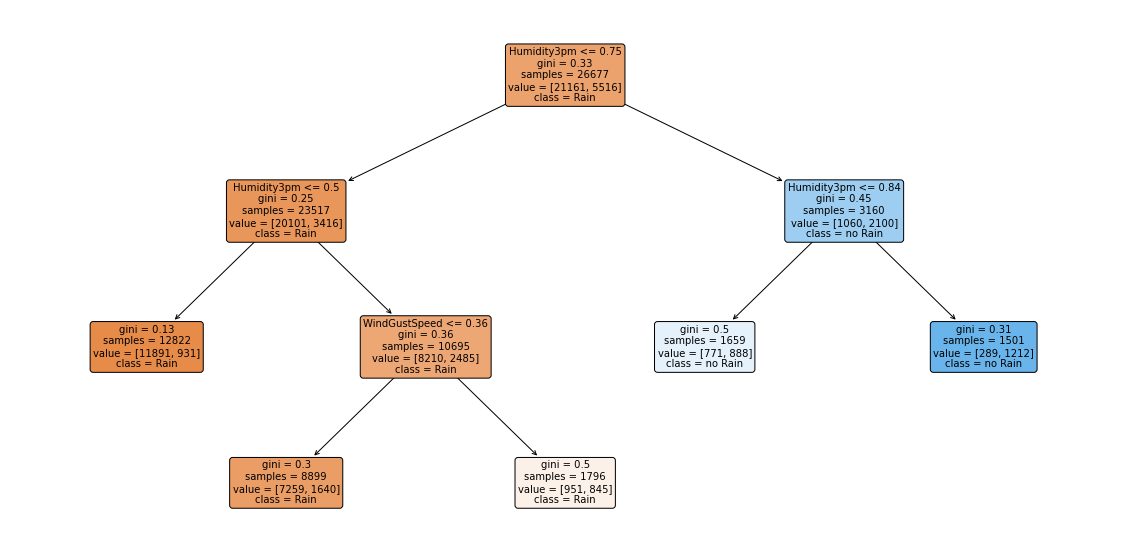
\includegraphics[width=0.9\textwidth]{Bilder/ccp_maxdepth_alpha_004.png}
        \caption{Entscheidungsbaum mit Parametern \emph{max\_depth=8} und \emph{ccp\_alpha=0.004}}
        \label{fig:ccp_maxDepth_alpha_004}
    \end{minipage}\hfill
\end{figure}
\pagebreak
\subsection{Quellcode zu Booklet Teil 1}
\pagebreak
\subsection{Quellcode zu Booklet Teil 2}
\pagebreak
\subsection{Quellcode zu Booklet Teil 3}
\pagebreak
\subsection{Quellcode zu Booklet Teil 4}